
\documentclass[border=0.125cm]{standalone}
\usepackage{tikz}
\usetikzlibrary{positioning}
\usepackage{ifthen}
\usetikzlibrary{matrix,arrows.meta,quotes,shadows,decorations.pathreplacing,positioning,fadings}
\usepackage{cfr-lm}

\colorlet{mewnol}{blue!75!cyan}%
\colorlet{allanol}{blue!50!black}%

\begin{document}
  \tikzset{%
		every neuron/.style={
			circle,
			draw,
			minimum size=1cm
		},
		neuron missing/.style={
			draw=none, 
			scale=4,
			text height=0.333cm,
			execute at begin node=\color{black}$\vdots$
		},
	}
	
	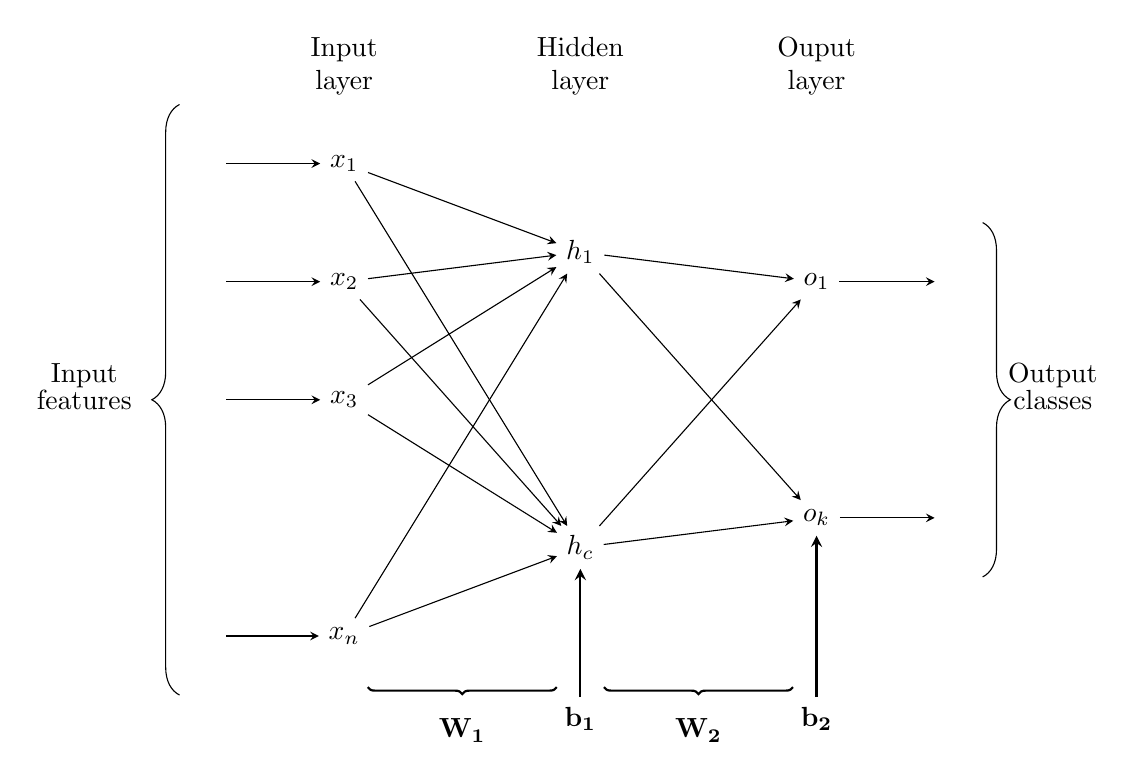
\begin{tikzpicture}[x=1.5cm, y=1.5cm, >=stealth]
	
	\foreach \m/\l [count=\y] in {1,2,3,missing,4}
	\node [every neuron/.try, neuron \m/.try] (input-\m) at (0,2.5-\y) {\ifthenelse{\equal{\m}{missing}}{}{\ifthenelse{\equal{\m}{4}}{$x_n$}{$x_\m$}} };
	
	\foreach \m [count=\y] in {1,missing,2}
	\node [every neuron/.try, neuron \m/.try ] (hidden-\m) at (2,2-\y*1.25) 
	{\ifthenelse{\equal{\m}{missing}}{}{\ifthenelse{\equal{\m}{2}}{$h_c$}{$h_\m$}} };
	
	\foreach \m [count=\y] in {1,missing,2}
	\node [every neuron/.try, neuron \m/.try ] (output-\m) at (4,1.5-\y) 
	{\ifthenelse{\equal{\m}{missing}}{}{\ifthenelse{\equal{\m}{2}}{$o_k$}{$o_\m$}} };
	
	\foreach \l [count=\i] in {1,2,3,n}
	\draw [<-] (input-\i) -- ++(-1,0)
	node [above, midway] {};
	
	\foreach \l [count=\i] in {1,h}
	\node [above] at (hidden-\i.north) {};
	
	\foreach \l [count=\i] in {1,n}
	\draw [->] (output-\i) -- ++(1,0)
	node [above, midway] {};
	
	\foreach \i in {1,...,4}
	\foreach \j in {1,...,2}
	\draw [->] (input-\i) -- (hidden-\j);
	
	\foreach \i in {1,...,2}
	\foreach \j in {1,...,2}
	\draw [->] (hidden-\i) -- (output-\j);
	
	\foreach \l [count=\x from 0] in {Input, Hidden, Ouput}
	\node [align=center, above] at (\x*2,2) {\l \\ layer};
	
	\node (bias-1) at (2, -3.2) {$\mathbf{b_1}$};
	\node (bias-2) at (4, -3.2) {$\mathbf{b_2}$};
	
	\draw [->, thick] (bias-1) -- (hidden-2);
	\draw [->, thick] (bias-2) -- (output-2);
	
  \draw [decorate,decoration={brace,amplitude=10pt},xshift=-4pt,yshift=0pt]
	(-1.3,-3.0) -- (-1.3,2.0) node [black,midway,xshift=-0.6cm] 
	{};
	
	\node (text-input-1) at (-2.2, -0.3) {Input}; 
	\node (text-input-2) at (-2.2, -0.5) {features}; 
	
	\draw [decorate,decoration={brace,amplitude=10pt, mirror},xshift= -4pt,yshift=0pt]
	(5.5,-2.0) -- (5.5,1.0) node [black,midway,xshift=-0.6cm] 
	{};
	
	\node (text-input-1) at (6, -0.3) {Output}; 
	\node (text-input-2) at (6, -0.5) {classes}; 
	
	\draw [
	thick,
	decoration={
		brace,
		mirror,
		raise=0.5cm
	},
	decorate
	] (0.2, -2.6) -- (1.8, -2.6);
	
	\node (w1) at (1.0, -3.3) {$\mathbf{W_1}$};
	
	\draw [
	thick,
	decoration={
		brace,
		mirror,
		raise=0.5cm
	},
	decorate
	] (2.2, -2.6) -- (3.8, -2.6);
	
	\node (w1) at (3.0, -3.3) {$\mathbf{W_2}$};
	
	\end{tikzpicture}
	
\end{document}